\documentclass{ximera}
\input{../../preamble}

\addPrintStyle{../..}

\begin{document}
	\author{Bart Lambregs}
	\xmtitle{Voorstelling en notatie}{}
    \xmsource\xmuitleg

Vectoren kunnen grafisch voorgesteld worden door een pijl.  
Een vector wordt altijd benoemd door bij de pijl een symbool van de vectoriële grootheid te zetten. 
Deze notatie gebeurt met één letter waarboven een pijltje wordt geplaatst. 
Zonder benoemen stelt de pijl geen vector voor (en kan het dus evengoed een echte pijl afgeschoten door een boog zijn)! De pijl geeft de drie variabele kenmerken weer, evenals het aangrijpingspunt.	


% INSERT TIKZ PICTURE RICHTING ZIN GROOTTE VAN VECTOR 


% HTML WERKT NIET VOOR DEZE TIKZ PICTURES 

\begin{image}
\begin{tikzpicture}
	% Draw the axes with arrows
	\draw[->] (-1,0) -- (5,0) node[right] {$x$};
	\draw[->] (0,-0.5) -- (0, 3) node[above] {$y$};
	
	\draw[->, thick, blue] (1,1) -- (3,2) node[midway, below right] {\(\vec{z}\)};
	\fill[blue] (1,1) circle (2pt) node[above left] {};
\end{tikzpicture}
\end{image}

\begin{image}
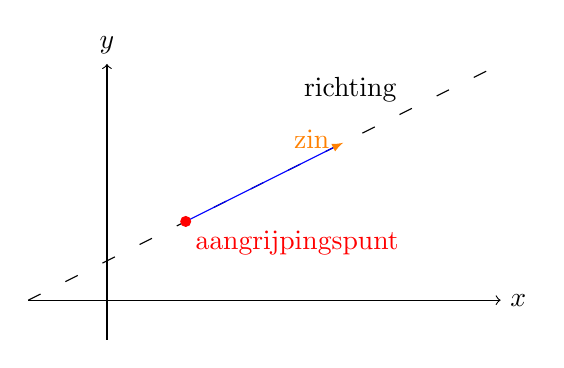
\begin{tikzpicture}
	% Draw the axes with arrows
	\draw[->] (-1,0) -- (5,0) node[right] {$x$};
	\draw[->] (0,-0.5) -- (0, 3) node[above] {$y$};
	
	% Draw the frame around the graphsp
	% \draw (0,0) rectangle (3,3);
	
	% Draw the vector with magnitude, direction, and point of application
	\draw[dash pattern=on 5pt off 10pt] (-1,0) -- (5,3) node[pos=0.80, above left] {richting};
	
	\draw[blue, -{latex[fill=orange]}] (1,1) -- (3,2) node[pos=0.80, above, orange] {zin};
	\fill[red] (1,1) circle (2pt) node[below right] {aangrijpingspunt};
	% \draw[thick, blue] (1,1) -- (3,2) node[midway, below right] {\(\vec{z}\)};
	
	
	% \draw[green, ->] (2.5,2.5) -- (2.75,2.75) node[right] {Magnitude};
	
	% Add the sense (arrowhead) in a separate color (e.g., purple)
	% \draw[thick, blue, -{>[scale=1.5, length=5pt, width=5pt, purple]}] (1,1) -- (2.5,2.5);
\end{tikzpicture}
\end{image}



% Tikz geprogrameerd zodat het een oefening kan zijn in lager jaar: bepaal aangrijpingspunt, richting, grootte en zin. 
\begin{tikzpicture}

	\draw (-5,-5) grid (5,5);


	\pgfmathsetmacro{\ax}{1}
	\pgfmathsetmacro{\ay}{1}
	\pgfmathsetmacro{\ex}{4}
	\pgfmathsetmacro{\ey}{2}
	
	\coordinate (O) at (0,0); %OORSPRONG 
	\coordinate (A) at (\ax,\ay);  % AANGRIJPINGSPUNT 
	\coordinate (E) at (\ex, \ey); % EINDPUNT 

	\draw[->, dashed] (E) -- ($(A) ! 1.5 ! (E) $) node[pos=1, above left]{richting};
	\draw[dashed] (A) -- ($(A) ! -0.5 ! (E) $);
	

	\draw[->,blue, very thick, -{latex[fill=orange]}] (A)--(E) 
		node[midway, above left, blue]{\(grootte \lvert \vec{z} \rvert \)}
		node[pos=1, above, orange]{zin};

	
	\fill[red] (A) circle (2pt) node[right]{(\ax, \ay)};
	\fill (O) circle (2pt) node[below right]{O};
\end{tikzpicture}


Aan de zin van een vector kan wiskundig een teken gekoppeld worden, dit hangt af van de gekozen referentie-as. 

+: in de zin van de gekozen referentie-as    -: tegen de zin van de referentie-as


De grootte van de vector wordt vaak als enkel positief aanzien (vooral in een situatie zonder referentie-as). 
Om dit te beklemtonen gebruikt men soms het normteken van de vector \( \lVert \vec{z} \rVert \) of het absolutewaardeteken van de grootte \(\lvert z \rvert \). 
Wanneer er echter geen twijfel is en de grootte sowieso positief is (zoals meestal bij krachten), noteert men ook gewoon \(z\). 

Enkele voorbeelden:


% INSERT TIKZ PICTURE ZWAARTEKRACHT EN ROLLENDE BAL 

De richting van een vector wordt soms ook weergegeven met een eenheidsvector \(\vec{e}\). Dit is een vector met een welbepaalde richting en met grootte gelijk aan \(1\). Het nut hiervan komt in formules tot uiting. Ook in de algebraïsche notatie kan men de drie kenmerken weergeven:


%  INSERT TIKZ NORM RICHTING ZIN ALGEBRAISCH 

\begin{remark}
Als de grootte van een vector \(\vec{c}\) gelijk is aan nul, noemt men dit ook de \textbf{nulvector}. 
Men noteert dit als: \(\vec{c} = \vec{0}\)   of  \( \lVert \vec{c} \rVert \)  of   \( c = 0 \)
Men mag niet noteren dat: \( \vec{c} = 0\)  
Linkerlid en rechterlid moeten immers beiden een scalar of beiden een vector zijn!
\end{remark}
	
\end{document}
